% answers.tex —— 2011 年·全国大纲卷·理科 · 参考答案与详细解析片段
% 由 tools/generate_projects.py 依来源总账自 2011/2011_数学真题_全国大纲理_试题.md + 2011/2011_数学真题_全国大纲理_解析正文.md + 2011/2011_数学真题_全国大纲理_答案要点.md 生成，勿手改（改源 MD 后重跑）


\begin{answer}
\gksolhead{1}{}

\textbf{题目}：

复数 $z=1+i$，$\overline z$ 为 $z$ 的共轭复数，则 $z\overline z-z-1=$\mbox{（　　）}

（A）$-2i$\quad（B）$-i$\quad（C）$i$\quad（D）$2i$

\Needspace{4\baselineskip}
\textbf{解析}

\Needspace{5\baselineskip}
$z\overline z=2$，所以
\nopagebreak[4]
\[
z\overline z-z-1=2-(1+i)-1=-i.
\]

选 B。

\gkanswer{答案：B}

\end{answer}
\begin{answer}
\gksolhead{2}{}

\textbf{题目}：

函数 $y=2\sqrt{x}$（$x\geq0$）的反函数为\mbox{（　　）}

（A）$y=\dfrac{x^2}{4}$（$x\in\mathbb R$）\quad（B）$y=\dfrac{x^2}{4}$（$x\geq0$）

（C）$y=4x^2$（$x\in\mathbb R$）\quad（D）$y=4x^2$（$x\geq0$）

\Needspace{4\baselineskip}
\textbf{解析}

交换 $x\text{、}y$ 得 $x=2\sqrt y$，所以
$y=x^2/4$，且反函数的定义域为 $x\geq0$，选 B。

\gkanswer{答案：B}

\end{answer}
\begin{answer}
\gksolhead{3}{}

\textbf{题目}：

下面四个条件中，使 $a>b$ 成立的充分而不必要的条件是\mbox{（　　）}

（A）$a>b+1$\quad（B）$a>b-1$\quad（C）$a^2>b^2$\quad（D）$a^3>b^3$

\Needspace{4\baselineskip}
\textbf{解析}

$a>b+1$ 必然推出 $a>b$，而 $a>b$ 不必推出
$a>b+1$，所以选 A。

\gkanswer{答案：A}

\end{answer}
\begin{answer}
\gksolhead{4}{}

\textbf{题目}：

设 $S_n$ 为等差数列 $\{a_n\}$ 的前 $n$ 项和，若 $a_1=1$，公差 $d=2$，$S_{k+2}-S_k=24$，则 $k=$\mbox{（　　）}

（A）$8$\quad（B）$7$\quad（C）$6$\quad（D）$5$

\Needspace{4\baselineskip}
\textbf{解析}

\Needspace{5\baselineskip}
$a_n=2n-1$，故
\nopagebreak[4]
\[
S_{k+2}-S_k=a_{k+1}+a_{k+2}
=(2k+1)+(2k+3)=4k+4.
\]

令 $4k+4=24$，得 $k=5$，选 D。

\gkanswer{答案：D}

\end{answer}
\begin{answer}
\gksolhead{5}{}

\textbf{题目}：

设函数 $f(x)=\cos\omega x$（$\omega>0$），将 $y=f(x)$ 的图象向右平移 $\dfrac\pi3$ 个单位长度后，所得的图象与原图象重合，则 $\omega$ 的最小值等于\mbox{（　　）}

（A）$\dfrac13$\quad（B）$3$\quad（C）$6$\quad（D）$9$

\Needspace{4\baselineskip}
\textbf{解析}

\Needspace{5\baselineskip}
$\pi/3$ 是函数的一个周期，所以
\nopagebreak[4]
\[
\frac\pi3=m\frac{2\pi}{\omega}\quad(m\in\mathbb N^+).
\]

因此 $\omega=6m$，最小值为 $6$，选 C。

\gkanswer{答案：C}

\end{answer}
\begin{answer}
\gksolhead{6}{}

\textbf{题目}：

已知直二面角 $\alpha-l-\beta$，点 $A\in\alpha$，$AC\perp l$，$C$ 为垂足，点 $B\in\beta$，$BD\perp l$，$D$ 为垂足。若 $AB=2$，$AC=BD=1$，则 $CD=$\mbox{（　　）}

（A）$\dfrac{\sqrt2}{3}$\quad（B）$\dfrac{\sqrt3}{3}$\quad（C）$\dfrac{\sqrt6}{3}$\quad（D）$1$

\Needspace{4\baselineskip}
\textbf{解析}

\Needspace{5\baselineskip}
取公共棱 $l$ 为 $x$ 轴，令
\nopagebreak[4]
\[
C=(0,0,0),\quad D=(\sqrt2,0,0),\quad
A=(0,1,0),\quad B=(\sqrt2,0,1).
\]
则 $AB=2$，且这些点满足题设的直二面角关系。平面
\Needspace{5\baselineskip}
$ABC$ 的一个法向量为
\nopagebreak[4]
\[
\overrightarrow{CA}\times\overrightarrow{CB}
=(1,0,-\sqrt2),
\]
\Needspace{5\baselineskip}
故
\nopagebreak[4]
\[
d(D,\text{\text{平面} }ABC)
=\frac{|(\sqrt2,0,0)\cdot(1,0,-\sqrt2)|}{\sqrt3}
=\frac{\sqrt6}{3}.
\]

选 C。

\gkanswer{答案：C}

\end{answer}
\begin{answer}
\gksolhead{7}{}

\textbf{题目}：

某同学有同样的画册 $2$ 本、同样的集邮册 $3$ 本，从中取出 $4$ 本赠送给 $4$ 位朋友，每位朋友 $1$ 本，则不同的赠送方法共有\mbox{（　　）}

（A）$4$ 种\quad（B）$10$ 种\quad（C）$18$ 种\quad（D）$20$ 种

\Needspace{4\baselineskip}
\textbf{解析}

若送出 $1$ 本画册，则选出收画册的朋友有
$\binom41=4$ 种；若送出 $2$ 本画册，则有
\Needspace{5\baselineskip}
$\binom42=6$ 种。因此总数为
\nopagebreak[4]
\[
\binom41+\binom42=4+6=10.
\]

选 A。

\gkanswer{答案：A}

\end{answer}
\begin{answer}
\gksolhead{8}{}

\textbf{题目}：

曲线 $y=e^{-2x}+1$ 在点 $(0,2)$ 处的切线与直线 $y=0$ 和 $y=x$ 围成的三角形的面积为\mbox{（　　）}

（A）$\dfrac13$\quad（B）$\dfrac12$\quad（C）$\dfrac23$\quad（D）$1$

\Needspace{4\baselineskip}
\textbf{解析}

曲线在 $(0,2)$ 处的导数为 $-2$，切线为
$y=-2x+2$。它与 $y=0$、$y=x$ 的交点分别为
\Needspace{5\baselineskip}
$(1,0)$、$(2/3,2/3)$，所以三角形面积为
\nopagebreak[4]
\[
\frac12\cdot1\cdot\frac23=\frac13.
\]

选 A。

\gkanswer{答案：A}

\end{answer}
\begin{answer}
\gksolhead{9}{}

\textbf{题目}：

设 $f(x)$ 是周期为 $2$ 的奇函数，当 $0\leq x\leq1$ 时，$f(x)=2x(1-x)$，则 $f\left(-\dfrac52\right)=$\mbox{（　　）}

（A）$-\dfrac12$\quad（B）$-\dfrac14$\quad（C）$\dfrac14$\quad（D）$\dfrac12$

\Needspace{4\baselineskip}
\textbf{解析}

\Needspace{5\baselineskip}
周期为 $2$ 且为奇函数，因此
\nopagebreak[4]
\[
f\left(-\frac52\right)=f\left(-\frac12\right)
=-f\left(\frac12\right)
=-\frac12.
\]

选 A。

\gkanswer{答案：A}

\end{answer}
\begin{answer}
\gksolhead{10}{}

\textbf{题目}：

已知抛物线 $C:y^2=4x$ 的焦点为 $F$，直线 $y=2x-4$ 与 $C$ 交于 $A\text{、}B$ 两点，则 $\cos\angle AFB=$\mbox{（　　）}

（A）$\dfrac45$\quad（B）$\dfrac35$\quad（C）$-\dfrac35$\quad（D）$-\dfrac45$

\Needspace{4\baselineskip}
\textbf{解析}

抛物线 $y^2=4x$ 的焦点为 $F=(1,0)$。直线与抛物线交于
$x=1$、$x=4$ 两点，可取
\Needspace{5\baselineskip}
$A=(1,-2)$、$B=(4,4)$。于是
\nopagebreak[4]
\[
\overrightarrow{FA}=(0,-2),\qquad
\overrightarrow{FB}=(3,4),
\]
\Needspace{5\baselineskip}
从而
\nopagebreak[4]
\[
\cos\angle AFB
=\frac{-8}{2\cdot5}=-\frac45.
\]

选 D。

\gkanswer{答案：D}

\end{answer}
\begin{answer}
\gksolhead{11}{}

\textbf{题目}：

已知平面 $\alpha$ 截一球面得圆 $M$，过圆心 $M$ 且与 $\alpha$ 成 $60^\circ$ 二面角的平面 $\beta$ 截该球面得圆 $N$。若该球面的半径为 $4$，圆 $M$ 的面积为 $4\pi$，则圆 $N$ 的面积为\mbox{（　　）}

（A）$7\pi$\quad（B）$9\pi$\quad（C）$11\pi$\quad（D）$13\pi$

\Needspace{4\baselineskip}
\textbf{解析}

\Needspace{5\baselineskip}
圆 $M$ 的半径为 $2$，故球心到平面 $\alpha$ 的距离为
\nopagebreak[4]
\[
d_\alpha=\sqrt{4^2-2^2}=2\sqrt3.
\]
平面 $\beta$ 经过 $M$，且与 $\alpha$ 成 $60^\circ$ 二面角，所以球心到
\Needspace{5\baselineskip}
$\beta$ 的距离为
\nopagebreak[4]
\[
d_\beta=d_\alpha\cos60^\circ=\sqrt3.
\]
圆 $N$ 的半径平方为 $16-3=13$，面积为 $13\pi$，选 D。

\gkanswer{答案：D}

\end{answer}
\begin{answer}
\gksolhead{12}{}

\textbf{题目}：

设向量 $\boldsymbol a\text{、}\boldsymbol b\text{、}\boldsymbol c$ 满足 $|\boldsymbol a|=|\boldsymbol b|=1$，$\boldsymbol a\cdot\boldsymbol b=-\dfrac12$，$\langle\boldsymbol a-\boldsymbol c,\boldsymbol b-\boldsymbol c\rangle=60^\circ$，则 $|\boldsymbol c|$ 的最大值等于\mbox{（　　）}

（A）$2$\quad（B）$\sqrt3$\quad（C）$\sqrt2$\quad（D）$1$

\Needspace{4\baselineskip}
\textbf{解析}

设 $\theta$ 为 $\boldsymbol a-\boldsymbol c$ 与
\Needspace{5\baselineskip}
$\boldsymbol b-\boldsymbol c$ 的夹角。由题设，
\nopagebreak[4]
\[
(\boldsymbol a-\boldsymbol c)\cdot
(\boldsymbol b-\boldsymbol c)
=|\boldsymbol a-\boldsymbol c|\,|\boldsymbol b-\boldsymbol c|
\cos60^\circ.
\]
直接将等式平方并利用
$|\boldsymbol a|=|\boldsymbol b|=1$、
\Needspace{5\baselineskip}
$\boldsymbol a\cdot\boldsymbol b=-1/2$，可得
\nopagebreak[4]
\[
|\boldsymbol c|^2-2
\leq0.
\]
等号可取，故 $|\boldsymbol c|_{\max}=2$，选 A。

\gkanswer{答案：A}

\end{answer}
\begin{answer}
\gksolhead{13}{}

\textbf{题目}：

$(1-\sqrt{x})^{20}$ 的二项展开式中，$x$ 的系数与 $x^9$ 的系数之差为\gkblank{}。

\Needspace{4\baselineskip}
\textbf{解析}

$(1-\sqrt x)^{20}$ 中 $x$ 项来自二项式的第 $2$ 项，系数为
$\binom{20}{2}=190$；$x^9$ 项来自第 $18$ 次取
$-\sqrt x$，系数为
$\binom{20}{18}=190$。两者之差为 $0$。

\gkanswer{答案：$0$}

\end{answer}
\begin{answer}
\gksolhead{14}{}

\textbf{题目}：

已知 $\alpha\in\left(\dfrac\pi2,\pi\right)$，$\sin\alpha=\dfrac{\sqrt5}{5}$，则 $\tan2\alpha=$\gkblank{}。

\Needspace{4\baselineskip}
\textbf{解析}

\Needspace{5\baselineskip}
$\alpha$ 在第二象限，故
\nopagebreak[4]
\[
\cos\alpha=-\frac2{\sqrt5},\qquad
\tan\alpha=-\frac12.
\]
\Needspace{5\baselineskip}
所以
\nopagebreak[4]
\[
\tan2\alpha
=\frac{2\tan\alpha}{1-\tan^2\alpha}
=-\frac43.
\]

\gkanswer{答案：$-\dfrac43$}

\end{answer}
\begin{answer}
\gksolhead{15}{}

\textbf{题目}：

已知 $F_1\text{、}F_2$ 分别为双曲线 $C:\dfrac{x^2}{9}-\dfrac{y^2}{27}=1$ 的左、右焦点，点 $A\in C$，点 $M$ 的坐标为 $(2,0)$，$AM$ 为 $\angle F_1AF_2$ 的平分线，则 $|AF_2|=$\gkblank{}。

\Needspace{4\baselineskip}
\textbf{解析}

双曲线的焦点为 $F_1=(-6,0)$、$F_2=(6,0)$，且
\Needspace{5\baselineskip}
$M=(2,0)$。由角平分线定理，
\nopagebreak[4]
\[
\frac{AF_1}{AF_2}=\frac{F_1M}{MF_2}=\frac84=2.
\]

$AF_1:AF_2=2:1$。又双曲线右支满足
$AF_1-AF_2=6$，故 $AF_2=6$。

\gkanswer{答案：$6$}

\end{answer}
\begin{answer}
\gksolhead{16}{}

\textbf{题目}：

已知点 $E\text{、}F$ 分别在正方体 $ABCD-A_1B_1C_1D_1$ 的棱 $BB_1\text{、}CC_1$ 上，且 $B_1E=2EB$，$CF=2FC_1$，则面 $AEF$ 与面 $ABC$ 所成的二面角的正切值等于\gkblank{}。

\Needspace{4\baselineskip}
\textbf{解析}

\Needspace{5\baselineskip}
设正方体棱长为 $1$，取
\nopagebreak[4]
\[
A=(0,0,0),\quad B=(1,0,0),\quad C=(1,1,0),
\]
并令 $B_1=(1,0,1)$、$C_1=(1,1,1)$。由
\Needspace{5\baselineskip}
$B_1E=2EB$、$CF=2FC_1$，得
\nopagebreak[4]
\[
E=\left(1,0,\frac13\right),\qquad
F=\left(1,1,\frac23\right).
\]
故平面 $AEF$ 的一个法向量可取
$\boldsymbol n=(-1,-1,3)$。与底面法向量
\Needspace{5\baselineskip}
$(0,0,1)$ 比较，二面角正切为
\nopagebreak[4]
\[
\tan\theta=\frac{\sqrt{(-1)^2+(-1)^2}}3
=\frac{\sqrt2}{3}.
\]

\gkanswer{答案：$\dfrac{\sqrt2}{3}$}

\end{answer}
\begin{answer}
\gksolhead{17}{}

\textbf{题目}：

$\triangle ABC$ 的内角 $A\text{、}B\text{、}C$ 的对边分别为 $a\text{、}b\text{、}c$。已知 $A-C=90^\circ$，$a+c=2b$，求 $C$。

\Needspace{4\baselineskip}
\textbf{解析}

设 $C=x$，则 $A=x+90^\circ$、$B=90^\circ-2x$。由正弦定理，
\Needspace{5\baselineskip}
$a+c=2b$ 化为
\nopagebreak[4]
\[
\cos x+\sin x=2\cos2x.
\]
\Needspace{5\baselineskip}
注意
\nopagebreak[4]
\[
\cos2x=(\cos x-\sin x)(\cos x+\sin x),
\]
\Needspace{5\baselineskip}
且 $\sin x+\cos x>0$，所以
\nopagebreak[4]
\[
\cos x-\sin x=\frac12.
\]
\Needspace{5\baselineskip}
平方后得 $\sin2x=3/4$。因 $0<2x<90^\circ$，故
\nopagebreak[4]
\[
C=x=\frac12\arcsin\frac34.
\]

\gkanswer{答案：$C=\dfrac12\arcsin\dfrac34$。}

\end{answer}
\begin{answer}
\gksolhead{18}{}

\textbf{题目}：

根据以往统计资料，某地车主购买甲种保险的概率为 $0.5$，购买乙种保险但不购买甲种保险的概率为 $0.3$。设各车主购买保险相互独立。

（1） 求该地 $1$ 位车主至少购买甲、乙两种保险中的 $1$ 种的概率；

（2） $X$ 表示该地的 $100$ 位车主中，甲、乙两种保险都不购买的车主数。求 $X$ 的期望。

\Needspace{4\baselineskip}
\textbf{解析}

\gksubpart{(1)}

\Needspace{5\baselineskip}
两种保险都不购买的概率为
\nopagebreak[4]
\[
1-0.5-0.3=0.2.
\]
所以至少购买一种保险的概率为 $1-0.2=0.8$。

\gksubpart{(2)}

\Needspace{5\baselineskip}
$X\sim B(100,0.2)$，因此
\nopagebreak[4]
\[
E(X)=100\cdot0.2=20.
\]

\gkanswer{答案（1）：至少购买一种保险的概率为 $0.8$。}

\gkanswer{答案（2）：$E(X)=20$。}

\end{answer}
\begin{answer}
\gksolhead{19}{}

\textbf{题目}：

如图，四棱锥 $S-ABCD$ 中，$AB\parallel CD$，$BC\perp CD$，侧面 $SAB$ 为等边三角形。$AB=BC=2$，$CD=SD=1$。
\nopagebreak[4]
\begin{center}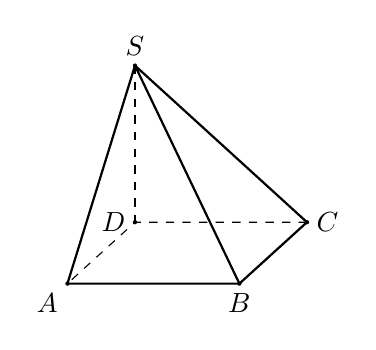
\begin{tikzpicture}[scale=.78,>=stealth]
\coordinate (A) at (0,0);
\coordinate (B) at (2.8,0);
\coordinate (C) at (3.9,1.0);
\coordinate (D) at (1.1,1.0);
\coordinate (S) at (1.1,3.55);
\draw[thick] (A)--(B)--(C);
\draw[dashed] (C)--(D)--(A);
\draw[thick] (S)--(A) (S)--(B) (S)--(C);
\draw[dashed] (S)--(D);
\fill (A) circle (1pt) node[below left] {$A$};
\fill (B) circle (1pt) node[below] {$B$};
\fill (C) circle (1pt) node[right] {$C$};
\fill (D) circle (1pt) node[left] {$D$};
\fill (S) circle (1pt) node[above] {$S$};
\end{tikzpicture}
\end{center}
\nopagebreak[4]
（1） 证明：$SD\perp$ 平面 $SAB$；

（2） 求 $AB$ 与平面 $SBC$ 所成角的正弦值。

\Needspace{4\baselineskip}
\textbf{解析}

\gksubpart{(1)}

\Needspace{5\baselineskip}
建立坐标系，取
\nopagebreak[4]
\[
A=(0,0,0),\quad B=(2,0,0),\quad
C=(2,2,0),\quad D=(1,2,0).
\]
设 $S=(1,u,v)$。由 $SAB$ 为边长 $2$ 的等边三角形，
$u^2+v^2=3$；又 $SD=1$，所以
\Needspace{5\baselineskip}
$(u-2)^2+v^2=1$，解得
\nopagebreak[4]
\[
S=\left(1,\frac32,\frac{\sqrt3}{2}\right).
\]
\Needspace{5\baselineskip}
于是
\nopagebreak[4]
\[
\overrightarrow{SD}=\left(0,\frac12,-\frac{\sqrt3}{2}\right),
\quad
\overrightarrow{AB}=(2,0,0),
\quad
\overrightarrow{AS}=\left(1,\frac32,\frac{\sqrt3}{2}\right).
\]
两点积分别为 $0$，故 $SD\perp$ 平面 $SAB$。

\gksubpart{(2)}

\Needspace{5\baselineskip}
平面 $SBC$ 的一个法向量为
\nopagebreak[4]
\[
\boldsymbol n=(\sqrt3,0,2),\qquad |\boldsymbol n|=\sqrt7.
\]
\Needspace{5\baselineskip}
所以
\nopagebreak[4]
\[
\sin\theta
=\frac{|\overrightarrow{AB}\cdot\boldsymbol n|}
{|\overrightarrow{AB}|\,|\boldsymbol n|}
=\frac{\sqrt3}{\sqrt7}
=\frac{\sqrt{21}}7.
\]

\gkanswer{答案（1）：见解析版}

\gkanswer{答案（2）：$AB$ 与平面 $SBC$ 所成角的正弦值为 $\dfrac{\sqrt3}{\sqrt7}=\dfrac{\sqrt{21}}7$。}

\end{answer}
\begin{answer}
\gksolhead{20}{}

\textbf{题目}：

\Needspace{5\baselineskip}
设数列 $\{a_n\}$ 满足 $a_1=0$ 且

\nopagebreak[4]
\[
\frac{1}{1-a_{n+1}}-\frac{1}{1-a_n}=1.
\]

（1） 求 $\{a_n\}$ 的通项公式；

（2） 设 $b_n=\dfrac{1-\sqrt{a_{n+1}}}{\sqrt n}$，记 $S_n=\displaystyle\sum_{k=1}^n b_k$，证明：$S_n<1$。

\Needspace{4\baselineskip}
\textbf{解析}

\gksubpart{(1)}

\Needspace{5\baselineskip}
令
\nopagebreak[4]
\[
\frac1{1-a_n}=u_n.
\]
递推式给出 $u_{n+1}=u_n+1$，而 $u_1=1$，故
\Needspace{5\baselineskip}
$u_n=n$，从而
\nopagebreak[4]
\[
a_n=1-\frac1n.
\]

\gksubpart{(2)}

\Needspace{5\baselineskip}
由上式
\nopagebreak[4]
\[
a_{n+1}=\frac n{n+1},
\]
\Needspace{5\baselineskip}
所以
\nopagebreak[4]
\[
b_n=\frac{1-\sqrt{n/(n+1)}}{\sqrt n}
=\frac1{\sqrt n}-\frac1{\sqrt{n+1}}.
\]
\Needspace{5\baselineskip}
因此
\nopagebreak[4]
\[
S_n=\sum_{k=1}^n b_k
=1-\frac1{\sqrt{n+1}}<1.
\]

\gkanswer{答案（1）：$a_n=1-\dfrac1n$。}

\gkanswer{答案（2）：见解析版}

\end{answer}
\begin{answer}
\gksolhead{21}{}

\textbf{题目}：

\Needspace{5\baselineskip}
已知 $O$ 为坐标原点，$F$ 为椭圆 $C:x^2+\dfrac{y^2}{2}=1$ 在 $y$ 轴正半轴上的焦点，过 $F$ 且斜率为 $-\sqrt2$ 的直线 $l$ 与 $C$ 交于 $A\text{、}B$ 两点，点 $P$ 满足

\nopagebreak[4]
\[
\overrightarrow{OA}+\overrightarrow{OB}+\overrightarrow{OP}=\boldsymbol0.
\]
\nopagebreak[4]
\begin{center}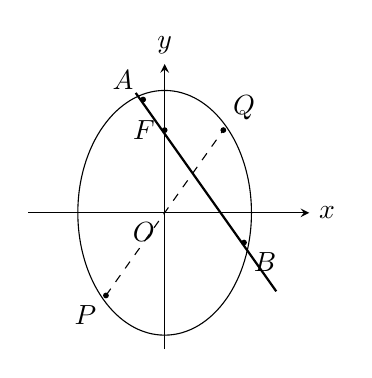
\begin{tikzpicture}[>=stealth,scale=1.05]
\draw[->] (-1.65,0)--(1.75,0) node[right] {$x$};
\draw[->] (0,-1.65)--(0,1.8) node[above] {$y$};
\draw (0,0) ellipse [x radius=1.05,y radius=1.48];
\draw[thick] (-.35,1.45)--(1.35,-.95);
\fill (-.26,1.37) circle (1pt) node[above left] {$A$};
\fill (.96,-.36) circle (1pt) node[below right] {$B$};
\fill (0,1) circle (1pt) node[left] {$F$};
\fill (-.71,-1) circle (1pt) node[below left] {$P$};
\fill (.71,1) circle (1pt) node[above right] {$Q$};
\draw[dashed] (-.71,-1)--(.71,1);
\node[below left] at (0,0) {$O$};
\end{tikzpicture}
\end{center}
\nopagebreak[4]
（1） 证明：点 $P$ 在 $C$ 上；

（2） 设点 $P$ 关于点 $O$ 的对称点为 $Q$，证明：$A\text{、}P\text{、}B\text{、}Q$ 四点在同一圆上。

\Needspace{4\baselineskip}
\textbf{解析}

\gksubpart{(1)}

椭圆方程为 $x^2+y^2/2=1$，其正焦点为
\Needspace{5\baselineskip}
$F=(0,1)$。直线 $l$ 为
\nopagebreak[4]
\[
y=1-\sqrt2x.
\]
\Needspace{5\baselineskip}
代入椭圆方程，交点横坐标满足
\nopagebreak[4]
\[
4x^2-2\sqrt2x-1=0.
\]
\Needspace{5\baselineskip}
故
\nopagebreak[4]
\[
x_A+x_B=\frac{\sqrt2}{2},\qquad
y_A+y_B=2-\sqrt2(x_A+x_B)=1.
\]
\Needspace{5\baselineskip}
由向量关系，
\nopagebreak[4]
\[
P=-(A+B)=\left(-\frac{\sqrt2}{2},-1\right),
\]
代入椭圆方程得 $P\in C$。

\gksubpart{(2)}

\Needspace{5\baselineskip}
令 $Q=-P=(\sqrt2/2,1)$。设过 $A\text{、}B$ 的圆为
\nopagebreak[4]
\[
x^2+y^2+Dx+Ey+F=0.
\]
\Needspace{5\baselineskip}
将直线 $y=1-\sqrt2x$ 代入，并与上面的交点二次方程比较系数，得
\nopagebreak[4]
\[
D-\sqrt2E=\frac{\sqrt2}{2},\qquad E+F=-\frac74.
\]
\Needspace{5\baselineskip}
再代入 $P\text{、}Q$，得到
\nopagebreak[4]
\[
D=\frac{\sqrt2}{4},\qquad E=-\frac14,\qquad F=-\frac32.
\]
\Needspace{5\baselineskip}
故 $P\text{、}Q$ 也在圆
\nopagebreak[4]
\[
x^2+y^2+\frac{\sqrt2}{4}x-\frac14y-\frac32=0
\]
上，四点共圆。

\gkanswer{答案（1）：见解析版}

\gkanswer{答案（2）：见解析版}

\end{answer}
\begin{answer}
\gksolhead{22}{}

\textbf{题目}：

（1） 设函数 $f(x)=\ln(1+x)-\dfrac{2x}{x+2}$，证明：当 $x>0$ 时，$f(x)>0$；

\Needspace{5\baselineskip}
（2） 从编号 $1$ 到 $100$ 的 $100$ 张卡片中每次随机抽取一张，然后放回，用这种方式连续抽取 $20$ 次，设抽得的 $20$ 个号码互不相同的概率为 $p$。证明：

\nopagebreak[4]
\[
p<\left(\frac9{10}\right)^{19}<\frac1{e^2}.
\]

\Needspace{4\baselineskip}
\textbf{解析}

\gksubpart{(1)}

\Needspace{5\baselineskip}
令
\nopagebreak[4]
\[
f(x)=\ln(1+x)-\frac{2x}{x+2}.
\]
\Needspace{5\baselineskip}
有
\nopagebreak[4]
\[
f'(x)=\frac1{x+1}-\frac4{(x+2)^2}
=\frac{x^2}{(x+1)(x+2)^2}>0\quad(x>0).
\]
又 $f(0)=0$，故 $f(x)>0$。

\gksubpart{(2)}

\Needspace{5\baselineskip}
抽取 $20$ 次且号码互不相同的概率为
\nopagebreak[4]
\[
p=\frac{100\cdot99\cdots81}{100^{20}}
=\prod_{k=1}^{19}\frac{100-k}{100}.
\]
\Needspace{5\baselineskip}
这 $19$ 个因子的算术平均数为 $0.9$，且它们不全相等，所以由算术—几何平均不等式，
\nopagebreak[4]
\[
p<\left(\frac9{10}\right)^{19}.
\]
\Needspace{5\baselineskip}
再由 $\ln(10/9)>2/19$，得
\nopagebreak[4]
\[
\left(\frac9{10}\right)^{19}<e^{-2}=\frac1{e^2}.
\]

\gkanswer{答案（1）：见解析版}

\gkanswer{答案（2）：见解析版}

\end{answer}